
The histogram by privatization is a optimized version of the naive strategy. The shortcomings of the naive strategy is the limited scalability caused by the thread contention in the atomic operation. The histogram by privatization tries to limit this shortcoming by decomposing the input data into smaller batches. An individually histogram is calculated by a thread block for each batch. The individually histograms is combined to created the final histogram. Doing the histogram calculation this way will limit the thread contention as the maximum amount of waiting threads are reduced from the input array size to amount of threads per block.
The individually thread blocks will besides the limited contention also benefit from the possible use of shared memory. Each thread block will create its own shared histogram, using shared memory and shared atomics. The usage of both shared memory and shared atomics will increase the performance. When each thread in a block is finished the private histogram is added to the global final histogram. For this addition there are two possible solution. Each solution is illustrated in \cref{fig:hist_privat}. 

\begin{figure}[ht]
	\centering
	\begin{subfigure}{0.9\textwidth}
		\centering
		\fbox{
			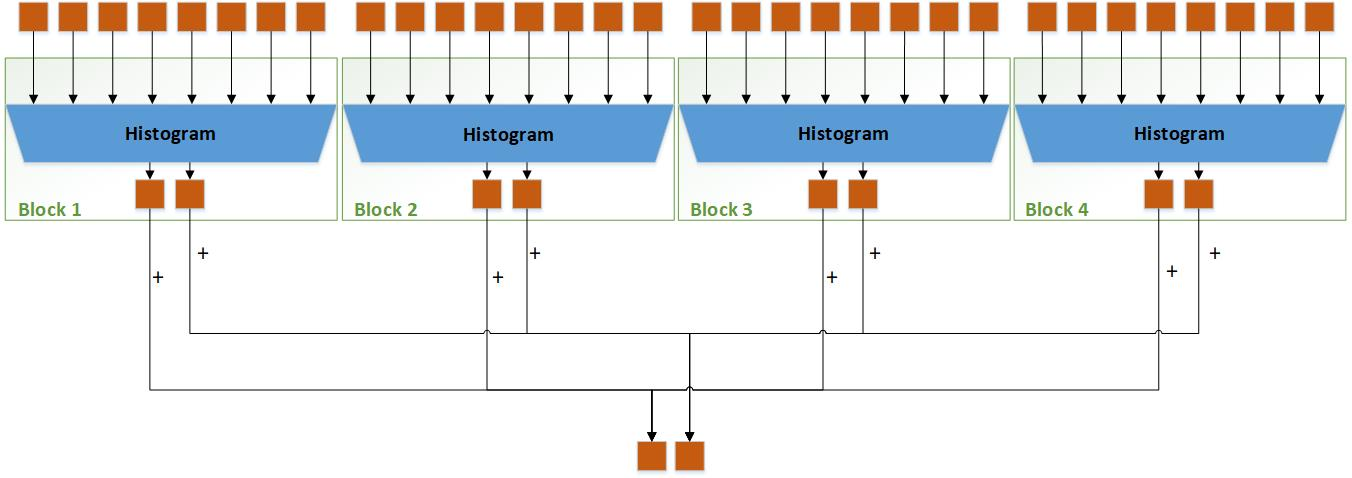
\includegraphics[width=0.9\textwidth]{figs/algorithm/hist_privat_atomic.jpg}}
		\caption{TBD}
		\label{fig:hist_privat_atomic}
	\end{subfigure}
	\begin{subfigure}{.9\textwidth}
		\centering
		\fbox{
			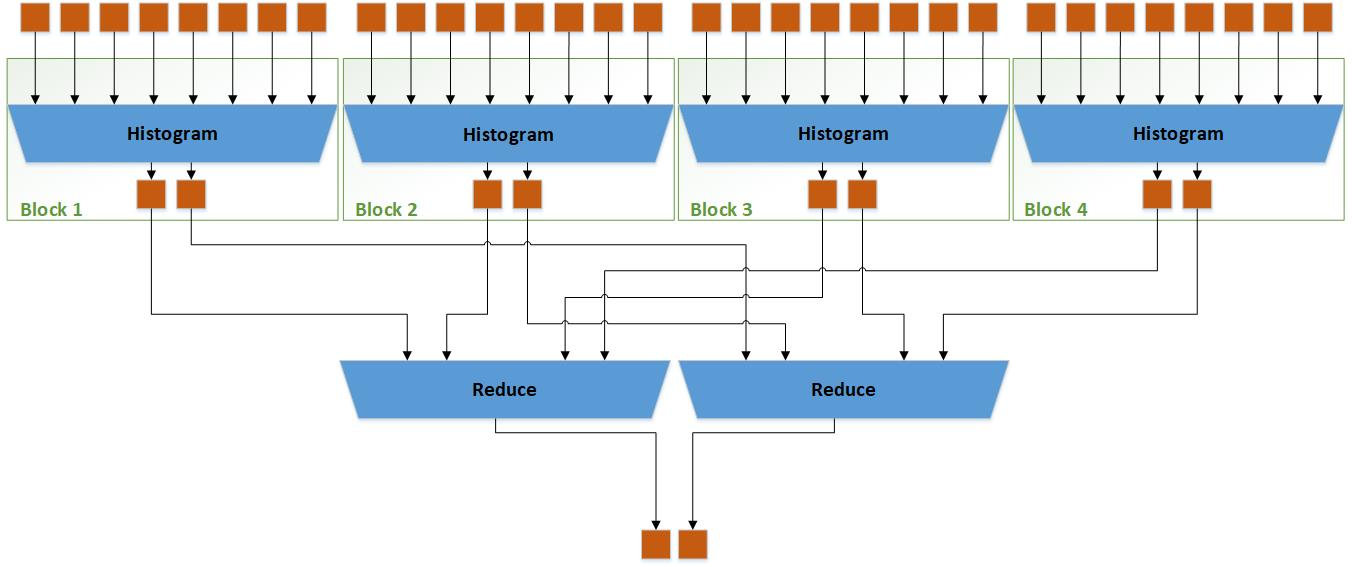
\includegraphics[width=0.9\textwidth]{figs/algorithm/hist_privat_reduce.jpg}}
		\caption{TBD}
		\label{fig:hist_privat_reduce}
	\end{subfigure}
	\caption{TBD}
	\label{fig:hist_privat}
\end{figure} 

The first addition solution as seen in \cref{fig:hist_privat_atomic} is to add the private histogram to the global histogram with atomics. As the naive and private  implementations the effectiveness of this solution is limited by the thread contention. The other solution, presented in \cref{fig:hist_privat_reduce} is to use the reduction algorithm from \cref{sec:al_reduction}. The reduction algorithm would be a good alternative to the atomic version, to avoid contention,  when there are many private histograms.       